\section{Experiments}\label{sec:experiments}
With an objective to improve designers' productivity in developing FPGA accelerators, the key goal
of QuickDough is to reduce FPGA loop accelerator development time for a hybrid CPU-FPGA system.
By using four typical loop kernels as the benchmark, we have evaluated the FPGA accelerator generation 
time with QuickDough. Meanwhile, to warrant the merit of such framework, the performance of the 
generated acceleration system should remain competitive. For that purpose, the performance is then 
compared against to that of software executed on an ARM processor. Finally, the pre-built accelerator 
library that affects both the design productivity and overhead of the resulting accelerators is also
discussed.

%The experiment section is organized as follows. We will first briefly introduce the benchmark programs in the following subsection and explain the basic experiment setup in \secref{subsec:setup}. Then we will discuss the accelerator library update in \secref{subsec:lib-update}. Finally, we will elaborate the loop accelerator generation time, performance and implementation overhead in \secref{subsec:acc-gen}, \secref{subsec:acc-perf} and \secref{subsec:acc-impl} respectively. 

\subsection{Benchmark} \label{subsec:benchmark}
Four applications were used as benchmark in this work, namely, a matrix-matrix multiplication (MM), a
finite impulse response (FIR) filter, a K-mean clustering algorithm (KM) and a Sobel edge detector
(SE). The basic parameters and configurations of the benchmark are illustrated in 
\tabref{tab:benchmark-config}. 

\begin{table}[htb]
    \centering
    \caption{Detailed Configurations of the Benchmark \label{tab:benchmark-config}}{
        \centering
        \resizebox{0.99\columnwidth}{!}{
            \begin{tabular}{l|l|l|l}
                \hline
                MM & FIR & SE & KM \\ \hline
                Matrix Size & \tabincell{l}{\# of Input/\\ \# of Taps+1} & \tabincell{l}{ \# of Vertical Pixels/\\ \# of Horizontal Pixels} & \tabincell{l}{\# of Nodes/Centroids/\\Dimension} \\ \hline
                100 & 10000/50 & 128/128 & 5000/4/2  \\ \hline
                1000 & 100000/50 & 1024/1024 & 50000/4/2 \\ \hline
            \end{tabular}
        }
    }
\vspace{-1em}
\end{table}

\subsection{Experiment Setup} \label{subsec:setup}
The Xilinx implementation tools were run on a computer with Intel Core i5-3230M CPU and
\SI{8}{\giga\byte} of RAM. The resulting HW-SW Co-design was targeted at 
Zedboard with both a hard ARM processor and an XC7Z020 FPGA. Software runtime was obtained 
from the ARM processor with -O3 compiling option. The accelerators were implemented on 
the FPGA of Zedboard. ISE 14.7 was used to implement the overlay based FPGA accelerators. 

The acceleration system handles the input data loading, accelerator computation and output data
storing sequentially. The performance of the accelerators is calculated using \eqnref{eq:comp-lat}
and \eqnref{eq:comm-lat} in \secref{sec:framework}. The data transfer latency used in
\eqnref{eq:comm-lat} is estimated based on Zedboard DMA between main memory and FPGA on-chip buffer
through AXI high-performance port. The
transfer latency is detailed in \tabref{tab:latency}. When the transfer size is not included in the
table, a simple linear model is used to estimate its latency. Fmax and the number of cycles were
extracted from the ISE14.7 and SCGRA scheduler respectively. 
 
\begin{table}
    \centering
    \caption{DMA transfer latency on Zedboard through AXI high performance port \label{tab:latency}}{
        \centering
        \resizebox{0.99\columnwidth}{!}{
            \begin{tabular}{c|c|c|c|c|c|c|c}
                \hline
                \tabincell{c}{transfer \\ size (word, 32bit)} & $\geq$512 & 256 & 128 & 64 & 32
                                                                  & 16 & $\leq$8  \\ \hline
                \tabincell{c}{Latency per \\ word (ns)}  & 10.08 & 11.28 & 13.32 & 15.18 & 21.45 & 36.24 & 63 \\ \hline
            \end{tabular}
        }
    }
\end{table}

Loop unrolling is a critical design input parameter for FPGA loop accelerators developed using QuickDough. It determines the parallelism that are exposed to the overlay architecture and influences the accelerator selection. While tuning the major accelerator design parameters together helps to achieve an optimized loop accelerator design, it requires more design efforts as detailed in \cite{scgra-customization} and it can be a complement to this work. \tabref{tab:unrolling-setup} shows the loop unrolling factors that are used for the loop accelerator generation.

\begin{table}
\footnotesize
\centering
\caption{QuickDough unrolling setup \label{tab:unrolling-setup}}{
    \resizebox{0.99\columnwidth}{!}{
        \begin{tabular}{l|l|l|l|l}
            \hline
           & MM & FIR & SE & KM \\ \hline
            Unrolling & $1 \times 5 \times 100$ & $50 \times 50$ & $16 \times 16 \times 3 \times 3$ &
            $125\times 4 \times 2$ \\ \hline
            DFG size & 750 & 2500 & 9720 & 5768 \\ \hline
            Full Loop & $100 \times 100 \times 100$ &  $10000 \times 50$ & $128 \times 128 \times 3
            \times 3$ & $5000 \times 4 \times 2$ \\ \hline
        \end{tabular}
    }
}
\end{table}

\subsection{Accelerator library update} \label{subsec:lib-update}
To ensure a rapid FPGA accelerator generation, we have implemented a group of 
SCGRAs based accelerators as the pre-built library by using the SCGRA overlay template. 
The library is developed to support all the four loop kernels, and it includes 12 
3-source-1-destination operations as presented in \tabref{tab:opset}. In addition, 
the pre-built accelerators share the same basic configurations as listed in 
\tabref{tab:scgra-config}.  

\begin{table}
    \centering
\caption{Operation Set. It covers all the four applications used in the experiments.
    \label{tab:opset}}{
\footnotesize 
\centering
\resizebox{0.6\columnwidth}{!}{
\begin{tabular}{l|c|l}
\hline
Type & Opcode & Expression \\

\hline
MULADD & 0001 & {Dst = (Src0 $\times$ Src1) + Src2} \\
\hline
MULSUB & 0010 & {Dst = (Src0 $\times$ Src1) - Src2} \\
\hline
ADDADD & 0011 & {Dst = (Src0 + Src1) + Src2} \\
\hline
ADDSUB & 0100 & {Dst = (Src0 + Src1) - Src2} \\
\hline
SUBSUB & 0101 & {Dst = (Src0 - Src1) - Src2} \\
\hline 
PHI & 0110 & {Dst = Src0 ? Src1 : Src2} \\
\hline
RSFAND & 0111 & {Dst = (Src0 $\gg$ Src1) \& Src2} \\
\hline
LSFADD & 1000 & {Dst = (Src0 $\ll$ Src1) + Src2} \\
\hline
ABS & 1001 & {Dst = abs(Src0)} \\
\hline
GT & 1010 & {Dst = (Src0 $>$ Src1) ? 1 : 0} \\
\hline
LET & 1011 & {Dst = (Src0 $\leq$ Src1) ? 1 : 0} \\
\hline
ANDAND & 1100 & {Dst = (Src0 \& Src1) \& Src2} \\
\hline
\end{tabular}
}
}
\end{table}

\begin{table}
\footnotesize 
\caption{SCGRA Configuration \label{tab:scgra-config}}{
\centering
  \resizebox{0.99\columnwidth}{!}{
\begin{tabular}{c|c|c|c|c}

\hline
{SCGRA Topology} & {\tabincell{c}{Instruction \\ Memory Width}} & {Data Memory} & {\tabincell{c}{I/O
Data \\ Buffer Width}} & {\tabincell{c}{I/O Addr \\ Buffer Width}} \\ \hline
{Torus} & {72 bits} & {$256 \times 32$ bits} & {32 bits} & {18 bits} \\ \hline
\end{tabular}
}
}
\end{table}

In addition, empirical settings are adopted to reduce the number of accelerators to be built in
library. Input and output buffer depth are set to be the same. The depth of the address buffers are
set to be twice with that of the I/O buffer depth. The data memory in each PE consumes only one
primitive block RAM. Instruction memory depth and I/O buffer depth are set to be $2^n$K $(n=0,1,2,
...)$. The SCGRA overlay adopts a torus topology, and the row size is set to be equal
to the column size or larger by one for the sake of performance. Eventually, different accelerator
configurations mainly differ on the on-chip I/O buffer depth, SCGRA size and instruction memory depth
when the data width is determined. 

To explore the library update process efficiency, we have evaluated the number of accelerators included in
the accelerator library and the time consumed to implement the library when different block RAM
budgets ranging from 70, 140, 210, 280 to 350 (Note that there are 140 RAMB36 on Zedboard FPGA) are
provided. As presented in \figref{fig:lib-impl-time}, when the BRAM budget increases, the number of accelerators
in the library and the library implementation time increase almost linearly. With a single
computer, the accelerator library implementation time ranges from 164 minutes to 3035 minutes.
However, with a cluster, the time cost of the highly parallel library implementation can decrease by
an order of magnitude easily.

\begin{figure}
\centering
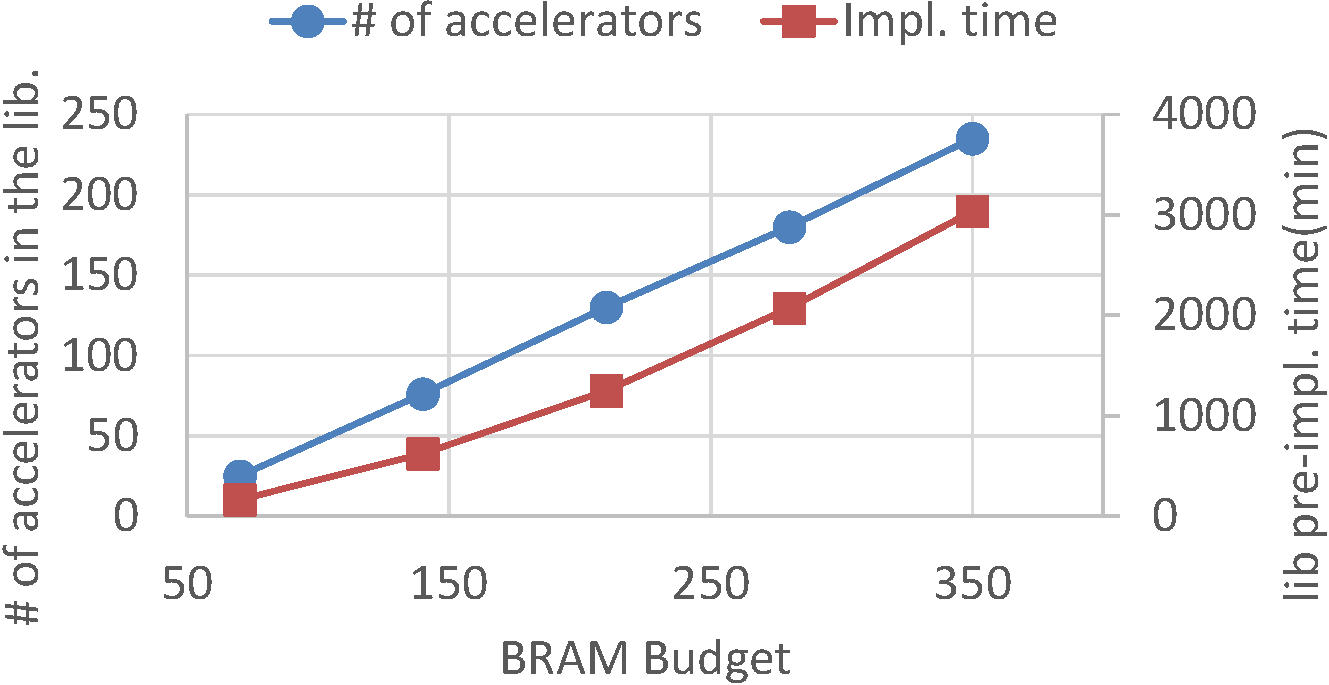
\includegraphics[width=0.75\linewidth]{lib-impl-time}
\caption{Accelerator library size and implementation time given different BRAM budgets.}
\label{fig:lib-impl-time}
\vspace{-1em}
\end{figure}

\subsection{Accelerator generation time} \label{subsec:acc-gen}
In this section, the loop accelerator generation time of QuickDough is evaluated. 
It is used as an indicator on the designer's productivity as it greatly limits 
the number of compile-debug-edit cycles achievable per day. 

In order to evaluate the loop accelerator generation time, we took the FPGA resource on Zedboard as
the resource budget and pre-built the accelerator library.
Then FPGA loop accelerators were generated for each application in the benchmark using the three
different accelerator selection options i.e. O0, O1 and O2.  
\tabref{tab:final-acc-config} shows the configurations of the resulting
FPGA accelerators as well as corresponding grouping factors. 

\begin{table}
\centering
\caption{Accelerators generated using QuickDough \label{tab:final-acc-config}}{
    \resizebox{0.95\columnwidth}{!}{
        \begin{tabular}{l|l|l|l|l|l}
            \hline
            \tabincell{c}{Opt. \\ option} & \tabincell{c}{Resulting \\ Config.} & MM & FIR & SE & KM \\ \hline
            \multirow{3}{*}{O0}  & SCGRA size & $2 \times 2$ & $2 \times 2$ & $2 \times 2$ & $2 \times 2$ \\ \cline{2-6} 
                                & Inst. Mem depth & 4K  & 4K & 4K & 4K \\ \cline{2-6} 
                                & I/O buffer depth & 4K & 4K & 4K & 4K \\ \cline{2-6}
                                & Grouping factor & 50x5x100 & 2500x50 & 128x64x3x3 & 1250x4x2 \\ \hline
            \multirow{3}{*}{O1}  & SCGRA size & $3 \times 3$  & $3 \times 3$  & $3 \times 3$  & $5
            \times 5$  \\ \cline{2-6} 
                                & Inst. Mem depth & 2K & 2K & 4K & 1K \\ \cline{2-6} 
                                & I/O buffer depth & 2K & 2K & 1K & 2K \\ \cline{2-6}
                                & Grouping factor & 25x5x100 & 1250x50 & 64x32x3x3 & 1000x4x2\\ \hline
            \multirow{3}{*}{O2}  & SCGRA size & $3 \times 3$ & $4 \times 4$  & $4 \times 4$  & $5
            \times 5$  \\ \cline{2-6} 
                                & Inst. Mem depth & 2K & 1K & 2K & 1K \\ \cline{2-6} 
                                & I/O buffer depth & 2K & 8K & 1K & 2K \\ \cline{2-6} 
                                & Grouping factor & 25x5x100 & 5000x50 & 64x32x3x3 & 1000x4x2 \\ \hline

        \end{tabular}
    }
}
\end{table}

With the pre-built library, every implementation iterations in QuickDough involves 3 steps:
\begin{itemize}[label=\textbullet,leftmargin=2em,rightmargin=\leftmargin]
\item DFG generation: The compute kernel is translated to corresponding DFG.
\item DFG scheduling: Select an accelerator configuration and schedule the DFG to it through an
    operation scheduling. 
\item Bitstream generation: The scheduling result is embedded into a pre-built accelerator bitstream 
to produce the final FPGA bitstream of the compute kernel.
\end{itemize}

\figref{fig:SCGRA-Overlay-Compilation-Time} shows loop accelerator generation time of QuickDough.
Both DFG generation and bitstream integration are very fast compared to the DFG scheduling step. The DFG
scheduling is relatively slower, but it usually completes in a few seconds.
Since the DFG scheduling process must be repeated when QuickDough explores different SCGRA size in
the accelerator library, the time consumption increases accordingly. Typically, the accelerator
generation time is relatively longer for more intensive accelerator selection. With O0 selection
where only a single DFG scheduling process targeting 2x2 SCGRA is needed, the accelerator can be
produced in less than 10 seconds. With O1 selection where three typical size of SCGRA (i.e. 2x2,
3x3, 5x5) will be evaluated, the accelerator
generation process completes in around half a minute. With the O2 selection where an exhaustive
search is performed, there are 76 accelerator configurations but only 7 different types of SCGRA
size are included in the library. 7 DFG scheduling processes are needed and the accelerator is
generated in one or two minutes.

\begin{figure}
\centering
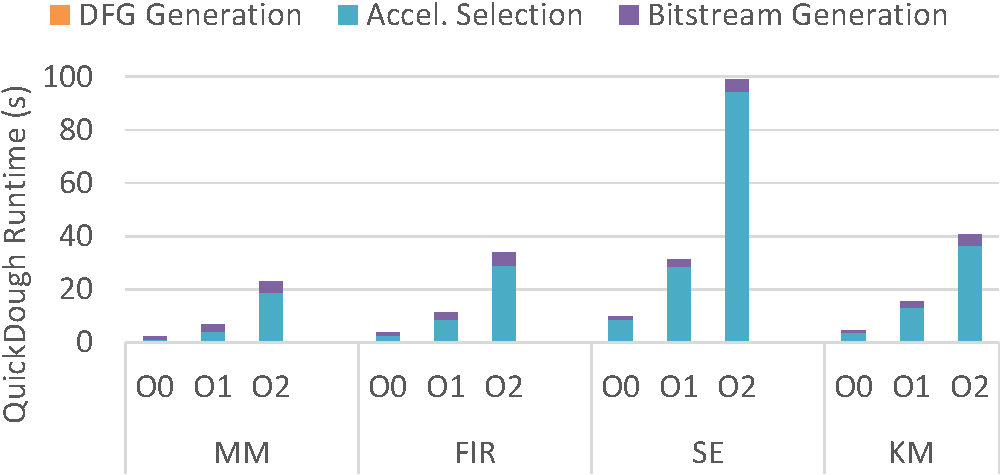
\includegraphics[width=0.85\linewidth]{quickdough-runtime}
\caption{Time consumption of loop accelerator generation using QuickDough.}
\label{fig:SCGRA-Overlay-Compilation-Time}
\end{figure}

Clearly, the designer must spend the time to physically pre-implement 
the overlay architecture on the target FPGA, spending considerable 
time on the implementation tools. However, it can be reused by the whole benchmark.
Moreover, the designer may iterate via the above rapid steps during 
design and debugging phases using an initial overlay implementation.
Once the functionality is frozen, the designer may then opt to further optimize 
performance through more intensive overlay customization and update the library. 
We argue that the ability to separate functionality and optimization 
concern, and the possibility of performing rapid debug-edit-implement 
iterations in QuickDough are crucial factors that contribute to a high-productivity 
design experience.

\subsection{Performance} \label{subsec:acc-perf}
While improving designers' productivity is the primary goal of QuickDough, the FPGA accelerators it
generates must remain competitive in performance to software executed on general 
purposed processors. Therefore, execution time of the loop kernels executed on ARM 
processor of Zedboard and FPGA accelerators generated using QuickDough are compared.

\figref{fig:real-perf} shows the accelerator performance speedup over software execution on the ARM processor 
and execution time decomposition of the 4 benchmark programs. The reported loop execution
time on the accelerators includes time spent on I/O data communication between FPGA and the 
ARM processor as well as FPGA computation.

\begin{figure}
\vspace{-1em}
\centering
\subfloat[MM]{
\label{fig:mm-real-perf}
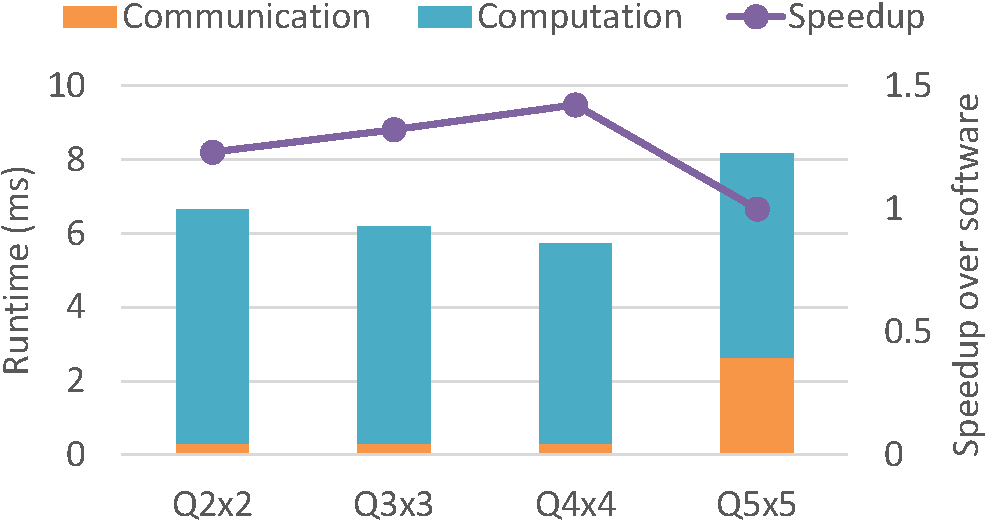
\includegraphics[width=0.44\linewidth]{mm-perf}}
\qquad
\subfloat[FIR]{
\label{fig:fir-real-perf}
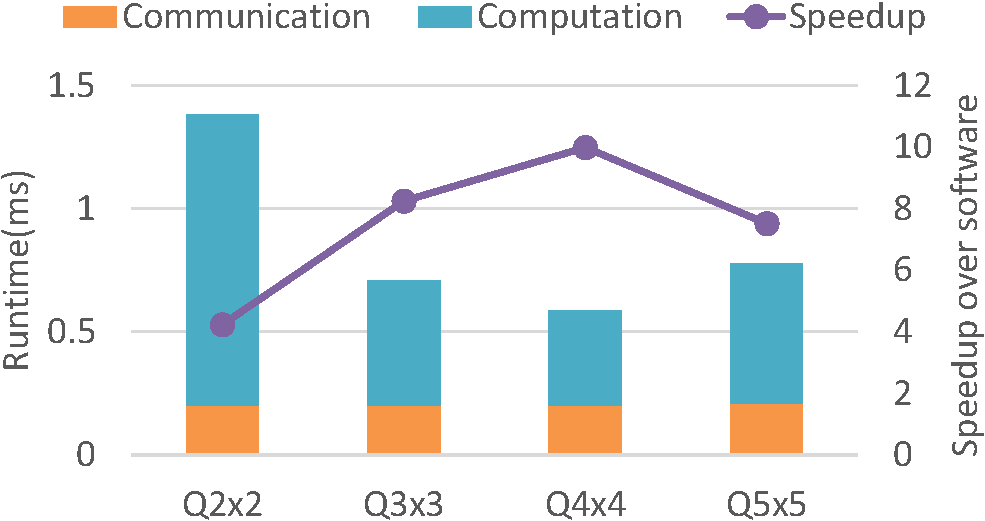
\includegraphics[width=0.44\linewidth]{fir-perf}}
\qquad
\subfloat[SE]{
\label{fig:sobel-real-perf}
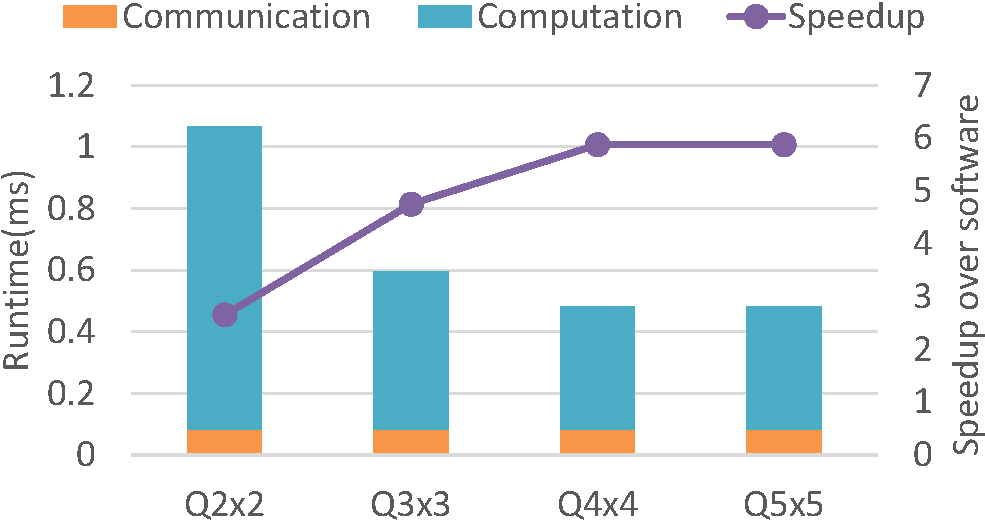
\includegraphics[width=0.44\linewidth]{se-perf}}
\qquad
\subfloat[KM]{
\label{fig:kmean-real-perf}
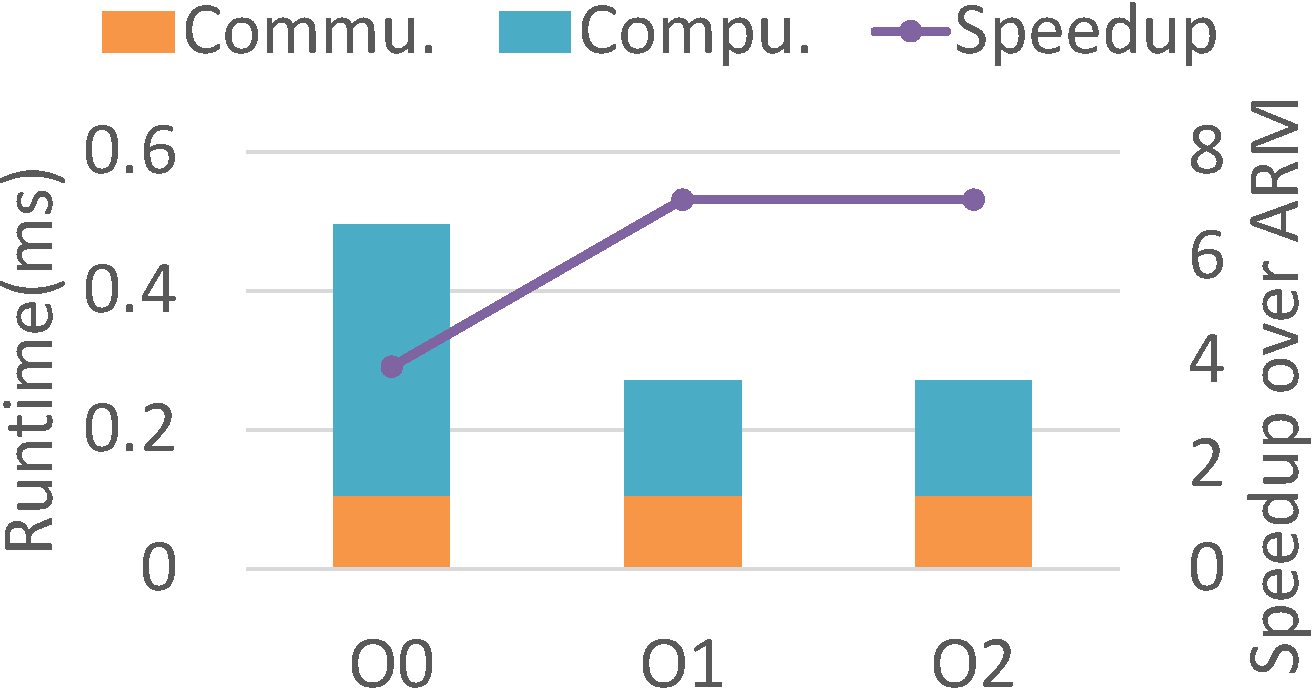
\includegraphics[width=0.44\linewidth]{km-perf}}
\caption{Benchmark performance speedup over software executed on ARM processor and execution time 
    decomposition of loop accelerators generated using QuickDough.}
\label{fig:real-perf}
\vspace{-1.2em}
\end{figure}

The results in \figref{fig:real-perf} show that the accelerators generated using QuickDough are 
capable to provide up to 9X performance speedup over software executed on ARM processor. For FIR, SE 
as well as KM which have abundant parallelism and moderate I/O requirements, the maximum speedup
goes up to 9X, 6X and 6X respectively. Even with simple acceleration selection and smallest SCGRA
size, clear performance speedup can be observed. MM optimized by simple loop unrolling is eventually reduced to
a matrix-vector multiplication, so the compute kernel has low compute-to-IO rate and the single port
connection between compute logic and input/output buffers becomes the bottleneck hindering
the performance of the accelerator.  

Accelerators with larger SCGRA overlay size typically achieve
better performance than the ones with smaller overlay size. However, larger SCGRA overlay will not
guarantee better performance for a few reasons. First of all, accelerators with larger overlay size consume
more block RAM for instruction memory leaving less block RAM for I/O buffer. As a result, the I/O
buffer may limit the transfer size between main memory and FPGA on-chip I/O buffer and reduce the
chance of data reuse between DFGs included in a single group. This increased number of transfer
between main memory and FPGA significantly limits the overall performance accordingly. Secondly, 
accelerator with larger SCGRA overlay may confront scheduling problem as larger SCGRA
overlay requires larger average cost between PEs and the compute performance may degrade as well.
Finally, larger SCGRA overlay based FPGA accelerators may result in lower implementation frequency
and degrade the overall performance as well. Optimal accelerators have the best trade-off on
buffering, scheduling and implementation frequency. According to \figref{fig:real-perf}, 3x3 or 4x4
SCGRA based FPGA accelerator achieve relatively better performance.

\subsection{Implementation frequency and hardware overhead} \label{subsec:acc-impl}
One advantage of employing a simple and regular overlay architecture allows highly 
pipelined implementations with much higher frequencies as shown in \figref{fig:impl-freq}. 
The increased running frequency in turns results in higher overall 
performance of the system. Though both larger SCGRA overlay size 
and deeper instruction memory may degrade the implementation frequency, the FMax of the
implementations is typically around 250MHz on Zedboard FPGA which is much higher than random logic
synthesis on Zedboard.

\begin{figure}[tb]
\vspace{-1em}
\center{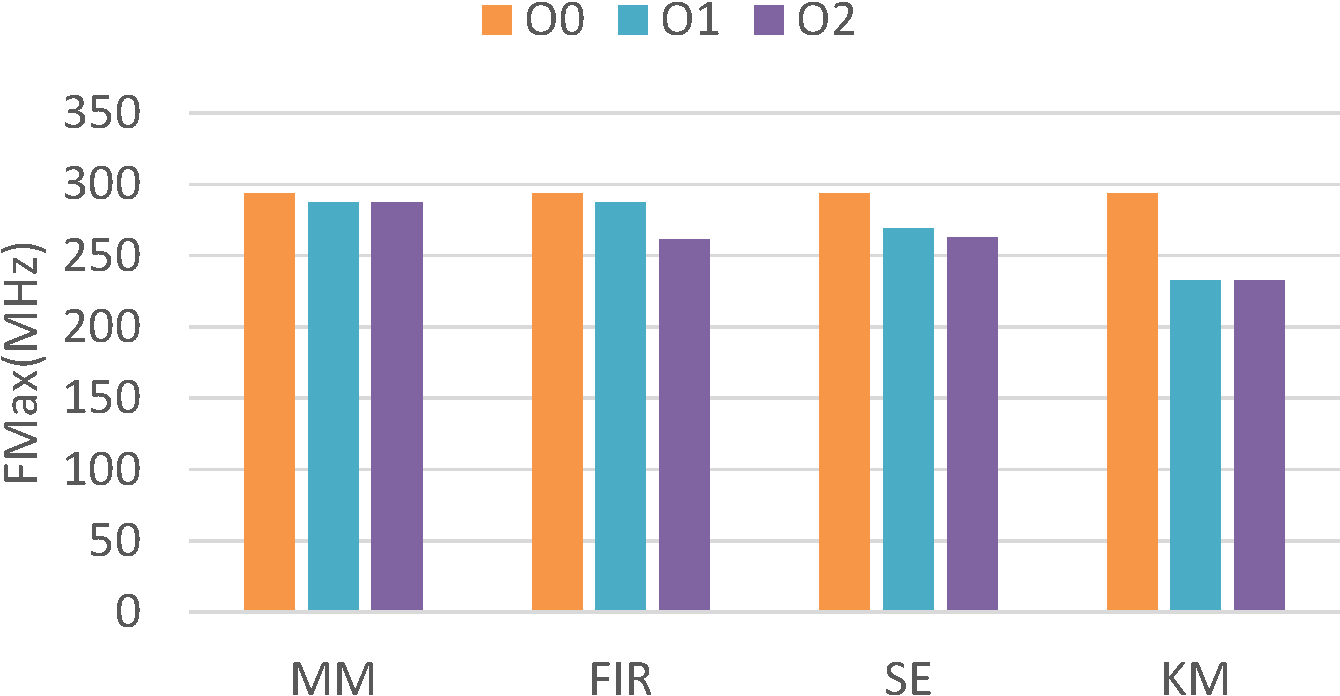
\includegraphics[width=0.65\linewidth]{impl-freq}}
\caption{Fmax of the accelerators generated using QuickDough}
\label{fig:impl-freq}
\end{figure}

As presented in \figref{fig:hw-overhead}, block RAM is the resource bottleneck for the SCGRA overlay
based FPGA accelerators. It may result in lower implementation frequency as the high utilization may
cause tight placing and routing. LUT, FF and DSP48 overhead mainly depends on the SCGRA overlay size and only a
portion of them are utilized.

\begin{figure}[tb]
\vspace{-0.5em}
\center{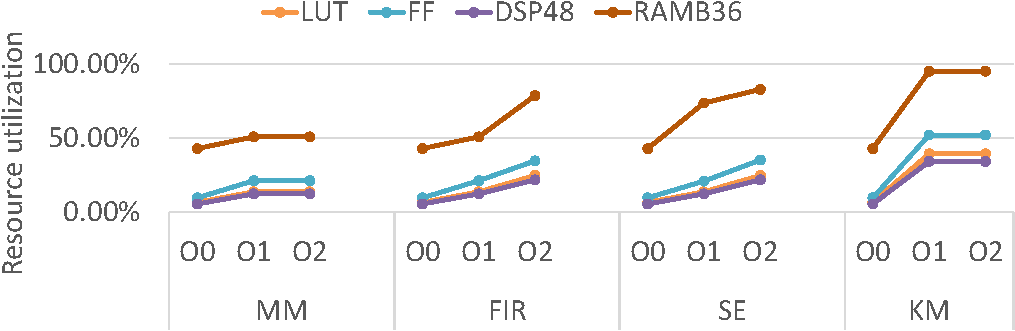
\includegraphics[width=0.8\linewidth]{hw-overhead}}
\caption{FPGA accelerator recource utilization}
\label{fig:hw-overhead}
\vspace{-1.2em}
\end{figure}


